\chapter{Literature Review}
\label{chap:lit-review}

This chapter provides a literature review of relevant past research efforts 
to give context to this dissertation. 
I begin with an overview of the \gls{FHR} concept, 
then go into detail about one specific \gls{FHR} design: the \gls{AHTR}, 
previous efforts and technical challenges of modeling the design, and a 
description of how these efforts led to the \gls{OECD} \gls{NEA}'s initiation 
of the \gls{FHR} benchmark.
Next, I outline additive manufacturing's history and describe the current 
research towards applying additive manufacturing to the fabrication of 
nuclear reactor components. 
I also review previous efforts towards nuclear reactor design optimization, 
describe how additive manufacturing of nuclear reactor components enables 
optimization for less constrained reactor geometries, and types of optimization 
methods, such as the evolutionary algorithm, that can be leveraged to find 
optimal reactor designs in the expanded design space.   
Finally, I give a background of the evolutionary algorithms and detail a specific 
evolutionary algorithm: the genetic algorithm and how it works to conduct global 
optimization robustly.

\section{Fluoride-Salt-Cooled High-Temperature Reactor System}
\label{sec:fhr}
To ensure continued global use and expansion of nuclear energy technology, in 
2001, the \gls{OECD} and nuclear energy experts initiated the \gls{GIF} 
\cite{gif_technology_2002}.
The \gls{GIF} aims to enhance the role of nuclear energy in our global energy 
ecosystem by coordinating global research and development to test the 
feasibility and performance of fourth generation nuclear systems, with the goal 
of making Gen IV reactors available for industrial deployment by 2030 
\cite{gif_technology_2002}.
The \gls{GIF} selected six Generation IV systems for further research and 
development based on target goals in four areas: sustainability, 
economics, safety and reliability, and proliferation resistance and physical 
protection \cite{gif_technology_2002}. 
Table \ref{tab:goals-gen4} summarizes the goals in each area. 
\begin{table}[btp]
    \centering
    \onehalfspacing
    \caption{Goals of Generation IV Nuclear Systems \cite{gif_technology_2002,
    behar_technology_2014}}
	\label{tab:goals-gen4}
    \footnotesize
    \begin{tabular}{l|l}
    \hline
                               \textbf{Area} & \textbf{Goals} \\ \hline
    Sustainability   & - Have a positive impact on the environment through the displacement of \\
    & polluting energy and transportation sources by nuclear electricity generation \\
    & and nuclear-produced hydrogen \\ 
    & - Promote long-term availability of nuclear fuel \\
    & - Minimize volume, lifetime, and toxicity of nuclear waste \\ \hline
    Economics & - Have a life cycle and energy production cost advantage over other energy \\
    & sources \\ 
    & - Reduce economic risk to nuclear projects by developing plants using \\
    & innovative fabrication and construction techniques \\ \hline
    Safety and Reliability   & - Increase the use of robust designs, and inherent and transparent safety\\
    & features that can be understood by non-experts \\ 
    & - Enhance public confidence in the safety of nuclear energy \\\hline
    Proliferation Resistance & - Provide continued effective proliferation resistance of nuclear energy \\
    and Physical Protection & systems through improved design features and other measures \\ 
    & - Increase the robustness of new facilities \\ \hline
    \end{tabular}
\end{table}
The systems are \glspl{GFR}, \glspl{LFR}, \glspl{MSR}, \glspl{SFR}, \glspl{SCWR}, 
and \glspl{VHTR} \cite{gif_technology_2002}. 
The \acrfull{FHR} concept introduced in 2003 uses a low-pressure liquid fluoride-salt 
coolant and high-temperature coated-particle \gls{TRISO} fuel, combining 
the best aspects of the \gls{MSR} and \gls{VHTR} systems respectively
\cite{forsberg_molten-salt-cooled_2003,facilitators_fluoride-salt-cooled_2013}.

\gls{MSR} systems produce fission power in a circulating molten salt fuel 
mixture. 
Researchers recommend molten fluoride salts because they have high uranium 
solubility, chemical stability, very low vapor pressure even at high 
temperatures, good heat transfer properties, resistance against radiation 
damage, and are inert to common structural materials 
\cite{rosenthal_molten-salt_1970}. 
Molten salt reactor coolants also introduce inherent safety due to the 
low system vapor pressure and the salts' high boiling temperature and 
volumetric heat capacity \cite{ho_molten_2013}.
Fluoride salt used in \glspl{FHR} is Li$_2$BeF$_4$ (FLiBe), 
which remains liquid without pressurization up to 1400 $^{\circ}$C and has a greater 
heat capacity than water \cite{ho_molten_2013,forsberg_fluoride-salt-cooled_2012}.
\gls{VHTR} systems use a once-through uranium cycle and leverage their 
high outlet temperature for high-temperature heat applications, such as 
hydrogen production. 
Graphite-moderated and helium-cooled, \glspl{VHTR} use \gls{TRISO} fuel
which withstands high burnup and temperature, enabling higher operating 
temperatures \cite{gif_technology_2002}.  
The advantages of higher operating temperatures include: increased power 
conversion efficiency, reduced waste heat generation, and co-generation and 
process heat capabilities \cite{scarlat_design_2014}.
However, the \glspl{VHTR} system's helium coolant is at 100 atm requiring a 
thick concrete vessel. 

By combining the FLiBE coolant from \gls{MSR} technology and 
\gls{TRISO} fuel from \gls{VHTR} technology, the \gls{FHR} benefits from 
a low operating pressure and large thermal margin enabled by the molten 
salt coolant and the thermal resilience of \gls{TRISO} particle fuel. 
Molten salt coolant's superior cooling properties compared to the \gls{VHTR}'s
helium coolant increases system safety with an atmospheric operating pressure 
instead of 100 atm. 
\gls{TRISO} solid fuel cladding in the \gls{FHR} system adds an extra barrier 
to fission product release compared to \glspl{MSR} with liquid fuel 
\cite{ho_molten_2013}.

Several types of \gls{FHR} conceptual designs exist worldwide: the \gls{PBFHR} 
developed at \gls{UCB} with circulating pebble-fuel 
\cite{scarlat_current_2014,krumwiede_three-dimensional_2013}, the \gls{SF-TMSR} 
developed at the \gls{SINAP} in China with static pebble-fuel \cite{liu_preliminary_2016}, 
the large central-station \gls{AHTR} at \gls{ORNL} \cite{holcomb_core_2011, varma_ahtr_2012} and 
the \gls{SmAHTR} at ORNL \cite{greene_pre-conceptual_2010} with static, plate fuel. 

\subsection{\acrlong{AHTR} Design}
This dissertation focuses on the prismatic \gls{FHR} design with hexagonal fuel 
assemblies consisting of \gls{TRISO} fuel particles embedded in planks, i.e., 
the \gls{AHTR} design developed by ORNL. 
The \gls{AHTR} has 3400 MWt thermal power and 1400 MW electric power with
inlet/outlet temperatures of 650/700$^{\circ}$C \cite{varma_ahtr_2012}.  
Figure \ref{fig:ahtr} shows the prismatic AHTR's fuel assembly and core 
configuration.  
\begin{figure}[btp]
    \centering
    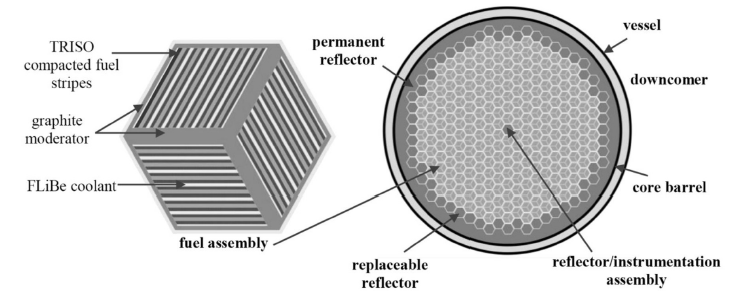
\includegraphics[width=\linewidth]{ahtr.png} 
    \caption{\acrlong{AHTR} fuel assembly (left) and core configuration (right) 
    reproduced from \cite{ramey_monte_2018}.}
    \label{fig:ahtr}
\end{figure}
Each hexagonal fuel assembly features plate-type fuel consisting of eighteen 
planks arranged in three diamond-shaped sectors, with a central Y-shaped 
structure and external channel (wrapper).
The fuel planks contain an isostatically pressed carbon with fuel stripes 
on each plank's outer side.
Within each fuel stripe is a graphite matrix filled with \gls{TRISO} particles. 
The core consists of 252 assemblies radially surrounded by reflectors
\cite{ramey_monte_2018}. 
Chapter \ref{chap:fhr-benchmark} details the specifications of the AHTR geometry
modeled in this proposed work.

\subsection{Previous AHTR modeling efforts and challenges} 
\label{sec:previous_ahtr}
The \gls{AHTR} core design differs significantly from the present \gls{LWR} 
systems' cores. 
These differences lead to modeling challenges with the current tools and also 
highlight the need for verification and validation of current simulation tools 
for \gls{AHTR} physics \cite{ramey_monte_2018}. 
Verification and validation of \gls{AHTR} neutronics and thermal-hydraulics 
simulation capabilities support the \gls{AHTR} design's licensure and 
eventual goal of \gls{AHTR} deployment 
\cite{rahnema_phenomena_2019,rahnema_current_2015}.
In this section, I outline the previous efforts taken to model and validate 
the \gls{AHTR}'s neutronics and thermal-hydraulics. 

\subsubsection{AHTR Neutronics Modeling}
Several neutronics studies conducted along the way to the current \gls{AHTR} 
design have shed light on the technical challenges facing the design 
\cite{ramey_monte_2018,holcomb_fluoride_2013,greene_pre-conceptual_2010}. 
\gls{Georgia Tech} led an Integrated Research Project to 
understand challenges in \gls{AHTR} materials and modeling its neutronics and 
thermal-hydraulics \cite{zhang_integrated_2019}. 
During the research project, a panel of subject matter experts 
generated a \gls{PIRT}.
The \gls{PIRT} identifies areas that need additional research to better 
understand important phenomena for adequate future modeling
\cite{rahnema_phenomena_2019}. 
Table \ref{tab:phenomena} lists the phenomena identified as requiring further 
research. 
\begin{table}[btp]
    \centering
    \onehalfspacing
    \caption{\acrlong{PIRT} identified \acrlong{AHTR} physical phenomena requiring 
    further research \cite{rahnema_phenomena_2019}.}
	\label{tab:phenomena}
    \footnotesize
    \begin{tabular}{l|l}
    \hline
    \textbf{Category} & \textbf{Phenomena} \\ \hline
    Fundamental cross section data & - Moderation in FliBe \\
    & - Thermalization in FliBe \\
    & - Absorption in FliBe \\
    & - Thermalization in carbon \\
    & - Absorption in carbon \\ \hline
    Material Composition & - Fuel particle distribution \\ \hline
    Computational Methodology & - Solution Convergence \\ 
    & - Granularity of depletion regions \\
    & - Multiple heterogeneity treatment for generating multigroup \\ 
    & cross sections \\
    & - Selection of multigroup structure \\
    & - Boundary conditions for multigroup cross section generation \\ \hline 
    General Depletion & - Spectral history \\ \hline 
    \end{tabular}
\end{table}

The \emph{triple heterogeneous} \gls{AHTR} fuel, comprised of \gls{TRISO} 
particles embedded in strategically arranged plates, presents simulation 
challenges. 
Researchers must obtain detailed reference power distributions with individual 
\gls{TRISO} particle fidelity to best understand nuances in the physics, such 
as self-shielding.
Deterministic codes that use multigroup cross sections and traditional 
homogenization methods \cite{ramey_monte_2018}, insufficiently capture the 
correct physics in \glspl{AHTR} due to these multiple heterogeneities
\cite{ramey_monte_2018}. 
In the \gls{AHTR}, single and multiple slab homogenization decreased total 
neutron transport simulation time by an order of 10; however, the homogenization 
introduced a nontrivial $k_{eff}$ error of $\sim$3\% 
\cite{ramey_monte_2018,cisneros_neutronics_2012}.
To determine the feasibility and safety of the \gls{AHTR} design, researchers 
must calculate core physics parameters to an acceptable uncertainty. 
With Monte Carlo neutron transport, increasing neutron histories reduces statistical 
uncertainty but increases computational cost typically, requiring the use of 
supercomputers to run the simulations.

This \gls{AHTR} presents another technical challenge: the uncertainty of 
graphite moderator material properties: densities, temperatures, and thermal 
scattering data.
Problematically, the thermal scattering data ($S(\alpha,\beta)$ matrices) for 
the bound nuclei in \gls{FLiBe} salts are lacking \cite{ramey_monte_2018}. 
Mei et al. \cite{mei_investigation_2013} and Zhu et al. \cite{zhu_thermal_2017} 
examined the thermal scattering behavior of solid and liquid \gls{FLiBe}.
They concluded that the bound and free atom cross section of \gls{FLiBe} are 
identical above 0.1eV and diverges below 0.01eV, which means that the use or 
absence of thermal scattering data will impact the accuracy of the results 
\cite{ramey_monte_2018}. 

\subsubsection{AHTR Multiphysics Modeling}
In past effort towards multiphysics modeling of the \gls{AHTR}, Gentry et al 
\cite{gentry_development_2016} developed an adapted lattice physics-to-core 
simulator two-step procedure with Serpent \cite{leppanen_serpent_2014} 
and \gls{NESTLE} \cite{turinsky_nestle_1994} for the \gls{AHTR} design. 
The adapted lattice physics-to-core simulator two-step procedure proved to be 
successful for \glspl{LWR} in which few group assembly homogenized group 
constants are generated by 2-D transport lattice calculation and then core 
analysis is performed by 3-D nodal simulation 
\cite{koebke_new_1980,gentry_development_2016}.
\gls{NESTLE}'s thermal-hydraulics utilizes a \gls{HEM} model for two-phase 
flow and it solves the few-group neutron diffusion equation utilizing the
\gls{NEM} for cartesian and hexagonal reactor geometries.  
Gentry et al concluded that the method required further accuracy improvements 
by improving reflector model and optimizing coarse energy group structure further.
Lin \cite{lin_thermal_2020} used RELAP5, a system-level code, to perform 
\gls{AHTR} thermal hydraulics transient simulations to investigate the 
capability of the passive heat removal system. 
In this \gls{AHTR} RELAP5 model, the 252 assemblies are separated into four 
concentric rings and a uniform power distribution is assigned to the fuel 
assemblies in each ring, and more fidelity is placed on the primary and 
\gls{DRACS} system loops. 
RELAP5 is a system-level code, Lin utilized it in transient scenarios to determine 
the temperature at various locations in the system loop by assuming a power 
value for fuel assemblies in each ring \cite{lin_thermal_2020}. 
However, this method is not ideal for transient scenarios with tightly coupled 
neutronics and thermal-hydraulics. 

\subsection{FHR Benchmark}
The previous section highlights the singular efforts to model 
different aspects of the \gls{AHTR}'s neutronics and thermal hydraulics, with
each author describing their modeling difficulties. 
However, there lacked a robust and methodical method for evaluating the 
simulation software and comparing the \gls{AHTR} modeling results generated by 
individual researchers.

To gain a wholistic view of the \gls{AHTR}'s modeling challenges and 
cross-verify available \gls{AHTR} modeling tools, in 2019, the 
\gls{OECD}-\gls{NEA} initiated the \gls{FHR} benchmarking exercise 
of the \gls{AHTR} design \cite{noauthor_fluoride_nodate}.
Several organizations participate in the benchmark with various Monte Carlo
and Deterministic neutronics software, such as Serpent \cite{leppanen_serpent_2014}, 
OpenMC \cite{romano_openmc_2013}, and WIMS \cite{lindley_current_2017}. 

The benchmark has three phases: a single fuel assembly simulation 
without burnup (Phase I), full core depletion (Phase II), and multi-physics 
feedback (Phase III). 
The benchmark aims to identify the applicability, accuracy, and practicality 
of the latest methods and codes to assess the current state 
of the art FHR simulation and modeling \cite{petrovic_preliminary_2021}. 
The benchmark also enables the cross-verification of software and methods 
for the challenging \gls{AHTR} geometry, which is especially useful since 
applicable reactor physics experiments for code validation are scarce 
\cite{petrovic_fhrahtr_2019,petrovic_preliminary_2021}. 
Chapter \ref{chap:fhr-benchmark} will provide a detailed description of the 
benchmark phases and results obtained so far.

\section{Additive Manufacturing}
Additive manufacturing is the formal term for what is popularly known as `3D printing' 
\cite{gibson_additive_2014}. 
The basic principle of additive manufacturing is that a model is initially generated using a
\gls{3D CAD} system and then fabricated directly without the need for process 
planning. 
Additive manufacturing, as the name implies, adds material in layers, such that 
each layer is a thin cross section of \gls{3D CAD}-designed part, as opposed 
to traditional machining which subtracts material instead 
\cite{standard_standard_2012}. 
All commercialized additive manufacturing machines to date use a layer-based approach, and 
the major ways that they differ are in materials, layer creation method, and 
how the layers are bonded to each other \cite{gibson_additive_2014}.
These major differences will determine the: accuracy of the 
final part, material and mechanical properties, time required to manufacture 
the part, need for post-processing, size of additive manufacturing machine, and overall 
cost of the machine and the process \cite{gibson_additive_2014}. 
Initially, industries only utilized additive manufacturing for manufacturing prototypes. 
However, with improvements in material properties, accuracy, and overall quality 
of additive manufacturing output, the applications for additive manufacturing expanded to the 
point at which some industries build parts for direct assembly purposes, such as
air-cooling ducts for aircrafts, hearing aids, and prosthesis
\cite{uriondo_present_2015}.  

Additive manufacturing has progressed rapidly in the last 30 years, from rapid 
design prototyping with polymers in the automotive industry to scale production 
of metal components.  
Examples include Boeing using additive manufacturing to reduce the 979 
Dreamliner's weight \cite{noauthor_printed_2017} and General Electric using 
additive manufacturing to produce fuel injection nozzles 
\cite{noauthor_transformation_2018}. 
The most common metal additive manufacturing technologies, \gls{SLM}, \gls{EBM}, 
\gls{L-DED}, and binder jetting, are not currently used to manufacture nuclear 
power plant parts. 

The U.S. \gls{DOE}, National Laboratories, \gls{EPRI} support research and 
development efforts towards deployment, testing, and qualification 
of additive manufacturing methods for nuclear components. 
However, the nuclear industry's efforts to incorporate additive manufacturing 
into the supply chain lags behind the auto and aerospace industries due to the 
lack of clarity on regulatory pathways. 
The aerospace and automotive industries benefit from long-standing and resourced 
regulatory and standards development activities \cite{noauthor_roadmap_nodate}. 
Thus, in 2019 the \gls{NRC} addressed these regulatory challenges by issuing 
a draft action plan to prepare the agency to review applications for 
additive manufacturing of nuclear components and clarify the industry's 
expectations of their use \cite{noauthor_roadmap_nodate}.

\subsection{Benefits of 3D Printing Reactor Components}
\label{sec:am}
Wide-spread adoption of additive manufacturing methods in the nuclear industry 
could drastically reduce fabrication costs and timelines.
These reductions are achieved by combining multiple systems and assembled 
components into single parts, tailoring local material properties and enabling 
geometry redesign for increased safety and performance 
\cite{simpson_considerations_2019}. 
Many Generation IV advanced reactor concepts have complex geometries, 
such as hex-ducts for sodium-cooled fast reactors, that are costly and difficult 
to fabricate using standard processing techniques \cite{sridharan_performance_2019}.  
These complex designs will benefit from 3D printed parts. 
Additive manufacturing advancements for reactor core components remove
conventional fuel manufacturing geometric constraints.
Reactor designers can now approach the nuclear design problems with truly 
arbitrary geometries, no longer limited by traditional geometric shapes that are 
easy to manufacture with traditional processes: slabs as fuel planks, cylinders 
as fuel rods, spheres as fuel pebbles, axis-aligned coolant channels, etc 
\cite{sobes_artificial_2020}.
In summary, reactor core component fabrication with additive manufacturing 
has the potential to enable further optimization and improvement of fuel 
geometries to enhance reactor performance at lower costs \cite{bergeron_early_2018}. 

\subsection{Efforts towards 3D Printing Reactor Components}
In 2019, \gls{ORNL} initiated the \gls{TCR} Demonstration Program.
The \gls{TCR} program leverages recent scientific achievements in additive 
manufacturing, nuclear materials, machine learning, and computational modeling
to reduce deployment costs and timelines for advanced nuclear energy systems. 
The \gls{TCR} program aims to utilize additive manufacturing technology to 
establish advanced nuclear energy system designs unconstrained by conventional 
manufacturing, and demonstrate the method's value by building an additively 
manufactured microreactor \cite{terrani_transformational_2019}. 

The \gls{TCR} program followed a downselection process based on the program's 
design contraints to select the reactor's design, materials, and components
\cite{betzler_transformational_2020}.
The downselected TCR design is a TRISO-fueled and yttrium hydride moderated 
gas-cooled reactor \cite{betzler_transformational_2020}.
At \gls{ORNL}, Trammel et al \cite{trammell_advanced_2019} demonstrated 
the fabrication of a SiC fuel element with embedded \gls{TRISO} fuel using 
additive manufacturing techniques: binderjet printing and \gls{CVI}. 
They followed the following fabrication steps (depicted in Figure 
\ref{fig:ornl-triso-print}): 
\begin{enumerate}
    \item A SiC fuel element with coolant channel structure is first printed with 
    binderjet technology. 
    \item The designated fueled region of the element is loaded with surrogate 
    \gls{TRISO} particles and additional SiC powder to fill interstitial spaces
    between particles. 
    \item The loaded fuel element is densified in a \gls{CVI} process to achieve 
    microencapsulation of \gls{TRISO} particles in a SiC matrix. 
\end{enumerate}
\begin{figure}[btp]
    \centering
    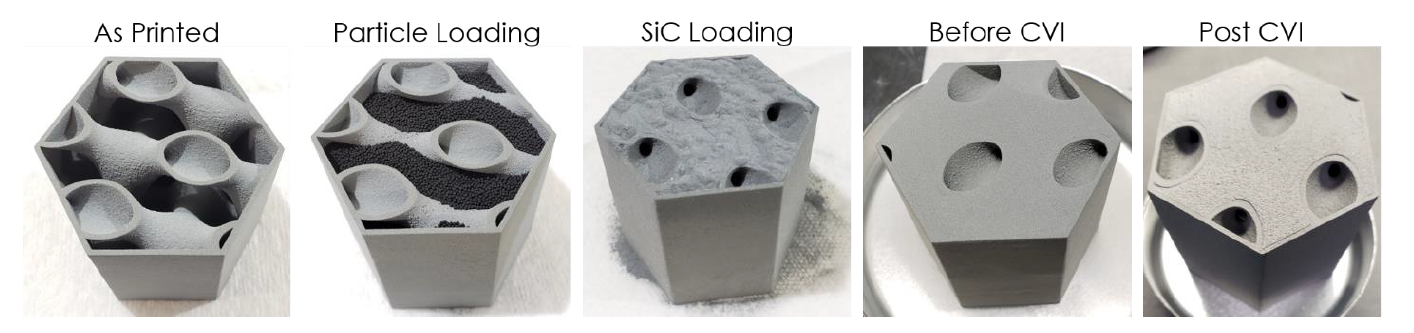
\includegraphics[width=\linewidth]{ornl-triso-print.png} 
    \caption{Stages of additive manufacturing fabrication conducted at \acrlong{ORNL} to 
    produce a fuel demonstration element with \gls{TRISO} particles embedded in 
    a SiC matrix \cite{trammell_advanced_2019}.}
    \label{fig:ornl-triso-print}
\end{figure}
Figure \ref{fig:ornl-fuel-element} shows the the fuel element manufactured at 
\gls{ORNL} for the \gls{TCR} program \cite{betzler_transformational_2020}. 
\begin{figure}[btp]
    \centering
    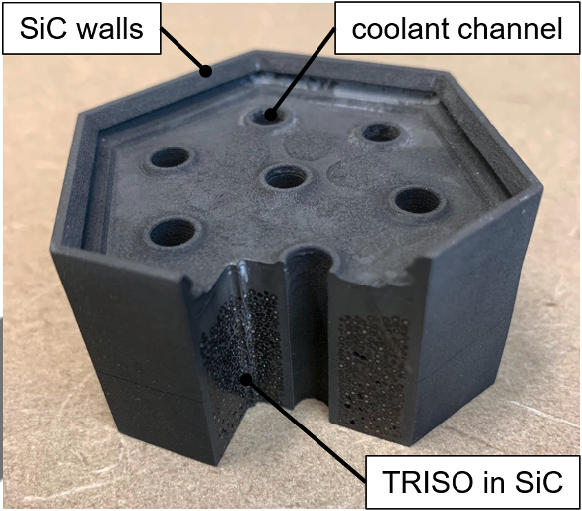
\includegraphics[width=0.6\linewidth]{ornl-fuel-element.png} 
    \caption{The top portion of the advanced manufactured fuel element 
    reproduced from \cite{betzler_transformational_2020} for the \acrfull{TCR} 
    program at \acrfull{ORNL}. A cutaway of the element shows surrogate TRISO 
    particles packed in the SiC matrix.}
    \label{fig:ornl-fuel-element}
\end{figure}
The current design uses fuel shapes and coolant channels that are uniform in the 
axial dimension. 
The \gls{TCR} programs plans to further optimize for coolant channels that vary 
in both axial and radial directions within the fuel element 
\cite{betzler_transformational_2020,sobes_artificial_2020}. 

Besides, the \gls{TCR} program, the nuclear materials research community has made 
significant progress in demonstrating the application of additive manufacturing 
to nuclear fuel and structural core material fabrication. 
Rosales et al. \cite{rosales_characterizing_2019} conducted a feasibility study 
of direct routes to fabricate dense uranium silicide (U$_3$Si$_2$) fuel pellets 
using the \gls{INL} approach known as \gls{AMAFT}. 
U$_3$Si$_2$ demonstrates desirable accident-tolerant nuclear fuel properties 
such as high uranium density and improved thermal properties, however, it has 
an expensive and long metallurgical fabrication process. 
Thus, using \gls{AMAFT} to fabricate U$_3$Si$_2$ will lower cost and ensure a
timely and commercially-reliable fabrication process \cite{rosales_characterizing_2019}. 
Sridharan et al. \cite{sridharan_performance_2019} demonstrated the application of
the laser-blown-powder additive manufacturing process to fabricate \gls{FM} steel, a type of 
steel commonly used for cladding and structural components in nuclear reactors. 
Koyanagi et al. \cite{koyanagi_additive_2020} presented the latest 
additive manufacturing technology for manufacturing nuclear-grade \gls{SiC} materials. 
They demonstrated that combinations of additive manufacturing techniques and 
traditional \gls{SiC} densification methods enabled new designs of \gls{SiC} 
components with complex shapes. 
\gls{SiC} demonstrates excellent strength at elevated temperatures, chemical inertness, 
relatively low neutron absorption, and stability under neutron irradiation up 
to high doses \cite{sauder_ceramic_2014, snead_handbook_2007,koyanagi_additive_2020}. 
These qualities make \gls{SiC} suitable for many applications in nuclear systems 
such as fuel cladding, constituents of fuel particles \cite{snead_handbook_2007} 
and pellets \cite{terrani_progress_2015}, and core structural components in fission 
reactors \cite{sauder_ceramic_2014}. 

% Advancements of nuclear material additive manufacturing technology 
% will enable 3D printing of nuclear reactors which will reduce the cost 
% and fabrication timelines. 

% The TCR Program's prototype demonstration of 3D printing a reactor shows promise 
% for the field.  

%Many of the materials and fabrication methods discussed above are applicable 
%for \gls{FHR}-part manufacturing. 
%Therefore, this reiterates the possibility of leveraging additive manufacturing 
%to 3D print a \gls{FHR}-type reactor with non-conventional geometry. 

\section{Nuclear Reactor Design Optimization}
\label{sec:opt}
A nuclear reactor's complexity results in reactor design optimization being a 
multi-objective design problem requiring a tradeoff between desirable 
attributes \cite{byrne_evolving_2014,simon_sciences_2019}. 
When multiple conflicting objectives compete no single optimum solution 
simultaneously optimizes all objectives. 
Instead, multi-objective optimization returns multiple optimal 
solutions that meets each objective to varying degrees, this is known as the 
Pareto front \cite{deb_multi-objective_2001}. 
For each solution in a set of Pareto front solutions, none of 
the objective functions can be improved in value without degrading some of the 
other objective values. 
For a multi-objective problem like reactor design, an ideal optimization method 
should find widely spread solutions in the obtained Pareto front 
\cite{deb_multi-objective_2001}. 

Traditional manufacturing constraints result in most of past nuclear reactor 
optimization work focusing on optimizing classical reactor 
parameters such as radius of fuel pellet and clad, enrichment of fuel, 
pin pitch, etc. 
The optimization methods used for reactor design optimization are either 
deterministic or stochastic methods. 
Deterministic optimization methods usually start from a guess solution.
Then, the algorithm suggests a search direction by applying local 
information to a pre-specified transition rule. 
Any better solution becomes the new solution, and the above procedure continues 
several times \cite{deb_multi-objective_2001}. 
Drawbacks of deterministic methods include: algorithms tend to get stuck at
suboptimal solutions, and an algorithm efficient in solving one type of problem 
may not solve a different problem efficiently \cite{deb_multi-objective_2001}. 
Stochastic optimization methods, such as evolutionary algorithms and simulated annealing,  
minimize or maximize an objective function when randomness is present. 
Stochasticity enables them to find globally optimal solutions more reliably than 
deterministic methods. 
Due to stochastic methods' many advantages, most efforts towards nuclear 
reactor optimization use these methods. 

In recent years, additive manufacturing advancements for reactor core components 
remove conventional fuel manufacturing geometric constraints such as slabs as fuel 
planks, cylinders as fuel rods, spheres as fuel pebbles, axis-aligned coolant 
channels, etc  \cite{sobes_artificial_2020}.
Reactor design objectives remain consistent with past objectives, such as 
minimizing fuel amount and minimizing the maximum fuel temperature for a given 
power level.
However, reactor designers can now approach the nuclear design problems with truly 
arbitrary geometries, and optimize beyond classical parameters to enhance 
fuel performance and safety further. 
This has opened the door for a re-examination of reactor core 
optimization in a completely new way, determining the optimal arbitrary geometry 
and fuel distribution for a given objective function with a much smaller set of 
constraints \cite{sobes_artificial_2020}. 

In the subsequent sections, I discuss the previous efforts towards nuclear 
reactor optimization for classical reactor parameters and arbitrary parameters. 

\subsection{Reactor Optimization for Classical Parameters}
The most commonly used stochastic optimization methods for reactor design 
optimization are simulated annealing and evolutionary algorithms. 

\subsubsection{Reactor Optimization with Simulated Annealing Method}
Simulated annealing iteratively updates one candidate solution until it reaches 
the termination criteria. 
At each iteration, the simulated annealing algorithm selects a random move. 
If the selected move improves the solution, it is always accepted; however,  
if it does not improve the solution, the algorithm updates the solution with 
some probability of less than 1.

Sacco et al. \cite{sacco_two_2006,sacco_metropolis_2008} used stochastic 
simulated annealing and deterministic-stochastic hybrid optimization techniques 
to optimize reactor dimensions, enrichment, materials, etc., to 
minimize the average peaking factor in a three-enrichment-zone reactor. 
Odeh et al. \cite{odeh_core_2016} used the simulated annealing stochastic algorithm 
coupled with neutronics and thermal-hydraulics simulation tools, \gls{PARCS} and RELAP5
\cite{fletcher_relap5mod3_1992}, to develop an optimal \gls{NMR-50} core design 
with a 10-year cycle length and minimal fissile loading. 
Kropaczek et al. \cite{kropaczek_large-scale_2019} demonstrated the constraint 
annealing method: a highly scalable method based on the method of parallel 
simulated annealing with mixing of states \cite{kropaczek_constraint_2019} for 
the solution of large-scale, multiconstrained problems in \gls{LWR} fuel cycle 
optimization. 
These papers demonstrate the simulated annealing optimization method's success in 
reactor design optimization problems. 

Nuclear reactor optimization problems require computationally 
expensive neutronics and thermal-hydraulics software to compute the objective 
function and constraints. 
Multiple papers utilized stochastic optimization methods with surrogate models 
and replace, high-fidelity neutronics or thermal hydraulics 
simulations to reduce computational cost.
Betzler et al. \cite{betzler_design_2019} developed a systematic approach to 
build a surrogate model to serve in place of high-fidelity computational 
analyses. 
They leveraged the surrogate model with a simulated annealing optimization 
algorithm to generate optimized designs at a lower computational cost and
understand the impact of design decisions on desired metrics for \gls{HFIR} \gls{LEU} 
core designs.

The simulated annealing method uses a point-by-point approach:
one solution gets updated to a new solution in one iteration, which does not 
exploit parallel systems' advantages.
Finding an optimal solution with simulated annealing methods takes very 
long if high-fidelity computationally expensive codes are used to compute 
the objective function and constraints.
Using a simulated annealing method is only practical if a 
surrogate evaluation model is used, as described in Betzler et al. 
\cite{betzler_design_2019}.

\subsubsection{Reactor Optimization with Evolutionary Algorithm Method}
Peireira et al. \cite{pereira_coarse-grained_2003,pereira_parallel_2008} 
used a coarse-grained parallel genetic algorithm and a niching genetic algorithm
to optimize the same problem as Sacco et al. \cite{sacco_two_2006}. 
Kamalpour et al. \cite{kamalpour_smart_2020} utilized the imperialist competitive 
algorithm, a type of evolutionary algorithm, to optimize a \gls{FCM} fuelled 
\gls{PWR} to extend the reactor core cycle length. 
Kumar et al. \cite{kumar_new_2015} combined genetic algorithm optimization 
with a surrogate model to optimize for high breeding of $^{233}$U and $^{239}$Pu 
in desired power peaking limits and keff by varying: fuel pin 
radius,  fissile material isotopic enrichment, coolant mass flow rate, and 
core inlet coolant temperature.

Contrary to a single solution per iteration in deterministic and stochastic 
simulated annealing methods, evolutionary algorithms use a population of solutions in each 
iteration \cite{deb_multi-objective_2001}. 
Evolutionary algorithm methods mimic nature's evolutionary principles to drive 
the search towards an optimal solution. 
With the affordability and availability of parallel computing systems, the 
evolutionary algorithm optimization method stands out as a method 
that easily and conveniently exploits parallel systems. 
Further, evolutionary algorithms have proved amenable to \gls{HPC} solutions and 
scalable to tens of thousands of processors \cite{kropaczek_constraint_2019}. 
Thus, for optimization problems that require high-fidelity evaluation software, 
the evolutionary algorithm method can leverage parallel computing to find a 
solution faster than the simulated annealing method.
Therefore, in this dissertation, I will utilize the evolutionary algorithm 
optimization method. 
Further literature review on evolutionary algorithms are described in Section 
\ref{sec:ea}.

\subsection{Reactor Optimization for Arbitrary Parameters}
Sobes et al \cite{sobes_artificial_2020} used a genetic algorithm to find 
minimum volume geometric configurations with multiphysics constraints of 
1500 pcm excess reactivity and maximum fuel temperature of 618 $^{\circ}C$ under 
forced-flow cooling conditions for a \gls{TCR}-like reactor. 
To represent arbitrary geometry variation, they constrained the solution geometry 
to right cylinders. 
The authors acknowledge that this work is only a first step towards truly 
arbitrary geometry expression. 
They found that the optimal cone-like core configuration is in the geometry 
shape of a truncated annular cone, with the inlet surface being larger than 
the outlet \cite{sobes_artificial_2020}.

See et al \cite{see_design_2022} conducted design optimization with Siemens 
design optimization tool HEEDS, and \gls{CFD} code, STAR-CCM+, to optimize the 
\gls{TCR}'s outlet plenum design. 
The design objectives were to normalize the fluidic temperature profile while 
maintaining a tight design constraint of 0.5-psi pressure drop. 

\section{Evolutionary Algorithms} 
\label{sec:ea}
With a substantial increase and change in an arbitrary geometry's design space, 
it becomes time consuming for a human reactor designer to thoroughly explore 
and find optimal geometries in the expanded design space. 
Instead, we can leverage \gls{AI} optimization methods, such as evolutionary 
algorithms, to promptly explore the large design space to find global optimal 
designs. 
\gls{AI} does not replace the human reactor designer but shifts the human 
designer's focus away from conjecturing suitable geometries to defining design 
criteria to find optimal designs \cite{sobes_artificial_2020}. 
Thus, when the human designer changes the reactor criteria, the \gls{AI} 
model will quickly adapt and produce new global optimal designs to fit the new 
criteria.  

Evolutionary algorithms, a subset of \gls{AI}, create a population of individual 
solutions, inspired by biological evolution, and induce goals by using a 
`fitness function' to mutate and preferentially replicate high-scoring 
individuals to reach an optimal solution.
Evolutionary algorithms often perform well at approximating solutions to many 
problem types because they do not make any assumptions about the 
underlying fitness landscape.
Genetic algorithms are the most popular evolutionary algorithms for solving 
multi-objective problems \cite{byrne_evolving_2014, krish_practical_2011}. 


\section{Summary}
This chapter provided a literature review of relevant past research 
efforts that give context to this dissertation. 
In summary, participation in the OECD-NEA FHR benchmarking exercise contributes 
to the assessment of the current neutron transport and thermal-hydraulics 
modeling and simulation capabilities for the \gls{AHTR} design.
Also, additive manufacturing of nuclear reactor components is a quickly 
developing field thanks to the aerospace and automotive industries, which led to 
breakthroughs in additive manufacturing fabrication of metal components. 
The promise of cheaper and faster manufacturing of reactor components with 
additive manufacturing frees complex reactor geometries from previous 
manufacturing constraints and allows reactor designers to reexamine reactor 
design optimization.  
Stochastic optimization methods such as evolutionary algorithms have proven to 
work well for finding global optimums in multi-objective design problems such as 
nuclear reactor optimization and can be leveraged to explore the vast exploration 
design space enabled by additive manufacturing.
